\documentclass[a4paper,norsk]{article}
\usepackage{preamble}

\begin{document}
\maketitle
\section*{Taylor-Green Vortex}

\section*{Abstract}

\section*{Physical problem}
The Taylor-Green vortex is a unsteady flow were we observe the flow of a decaying
vortex. This flow has an exact solution for the incrompessible Navier-Stokes equation in 2D, while for the 3D
case there are several numerical results for comparison.
Assuming the fluid is incompressible, the exact solution for velocity and pressure are given as

\begin{align}
u(x,y,t) = (cos(\pi x)sin(\pi y) e^{-2 t \nu \pi^{2} }, cos(\pi y)sin(\pi x) e^{-2 t \nu \pi^2} ) \\
p(x,y,t) = -0.25(cos(2\pi x) + cos(2 \pi y) ) e^{-4 t \nu \pi^2}
\end{align}


For the 3D case we will consider the kinetic energy for the system defined by $E_k = \frac{1}{2}||u||^2_{L^2}$

\section*{Governing Equation and Computations}
The incompressible Naiver-Stokes equation describes the flow motion, from the principles of conservation of momentum
and continuum.

\begin{align}
&\frac{\partial \textbf{v}}{\partial t} + \textbf{v} \cdot \nabla \textbf{v} =
-\nabla p + \nu \nabla^2 \textbf{v} \\
&\nabla \cdot \textbf{v} = 0
\end{align}

There is a open sea full of different approaches to solve this non-linear equation. We will for this
time explore Chorins method, and the incremental pressure correction scheme (\textit{IPCS}).

We will use the FEniCS project, a open-source PDE solver using the finite element method approach.
As verification of our solvers, the known analytical solution for the 2D Taylor-Green Vortex will be used as comparison.

The Reynolds number, discovered Osborne Reynolds as the relation between inertial and viscous forces, is defined
as
\begin{align}
Re = \frac{\rho U_{0} D}{\mu} = \frac{U_{0} D}{\nu}
\end{align}
Where $\nu$ denotes the kinematic viscosity, while $U_{0}$ and \textit{D} is some characteristic velocity and lenght.
For this problem a

\section*{Setting up 2D problem}

For the 2D case, the computational domain is set as $\Omega \in [-1, 1]^2$. Further on we will set
the flow conditions as \\

\begin{tabular}{l*{6}{c}r}
Physical Quantity              & Value  \\
\hline
Reynolds Number, Re & 1000   \\
Characteristic length, L           & 2     \\
Characteristic velocity, $U_{0}$   & 1     \\
Time step $\Delta t$ 			   & 0.001 \\
End time, T 					   & 1.0
\end{tabular}

Using our analytical solution for time $t = 0$, we set up the initial condition
for the domain $\Omega$

\begin{figure}[h!]
	\centering
	\caption*{Initial velocity field}
	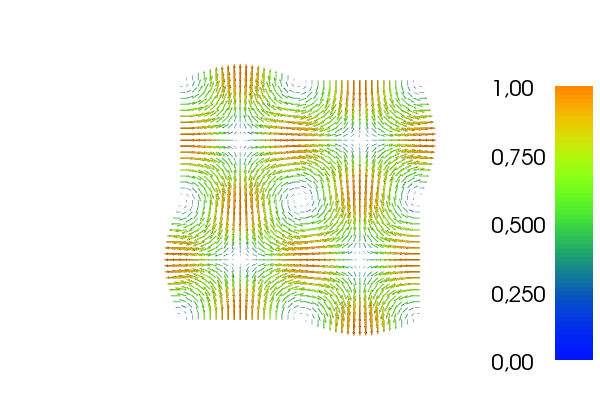
\includegraphics[scale=0.32]{2D/initial.png}
    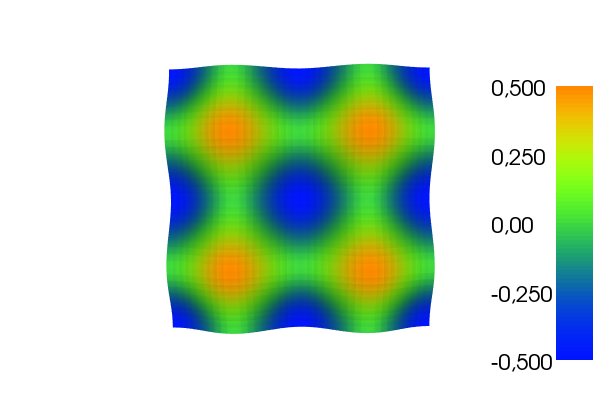
\includegraphics[scale=0.32]{2D/initpress.png}
\end{figure}


\section*{Results}
2D case Oasis Runtime: 3.8886 \\

Chorin own implementation 7.039

\begin{figure}[h!]
	\centering
	\caption*{Kinetic Energy}
	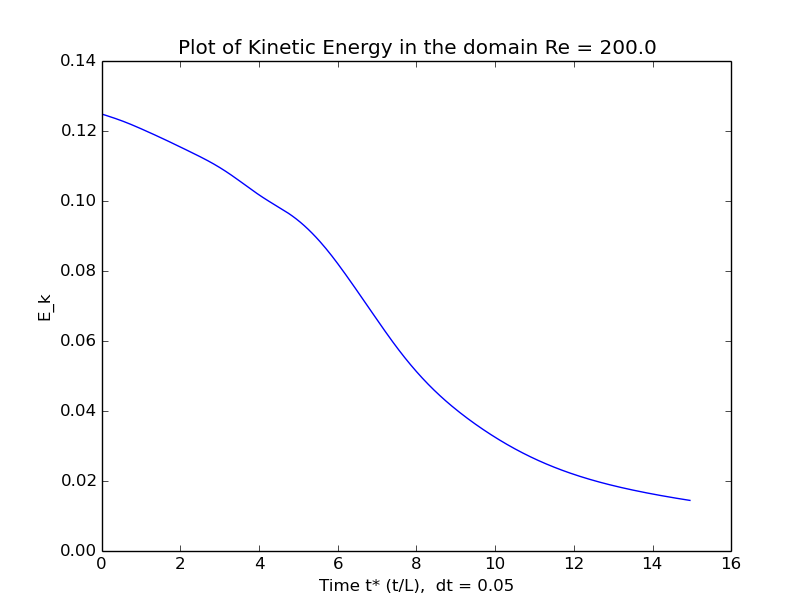
\includegraphics[scale=0.6]{3D/Et.png}
\end{figure}

\begin{figure}[h!]
	\centering
	\caption*{Dissipation Energy}
	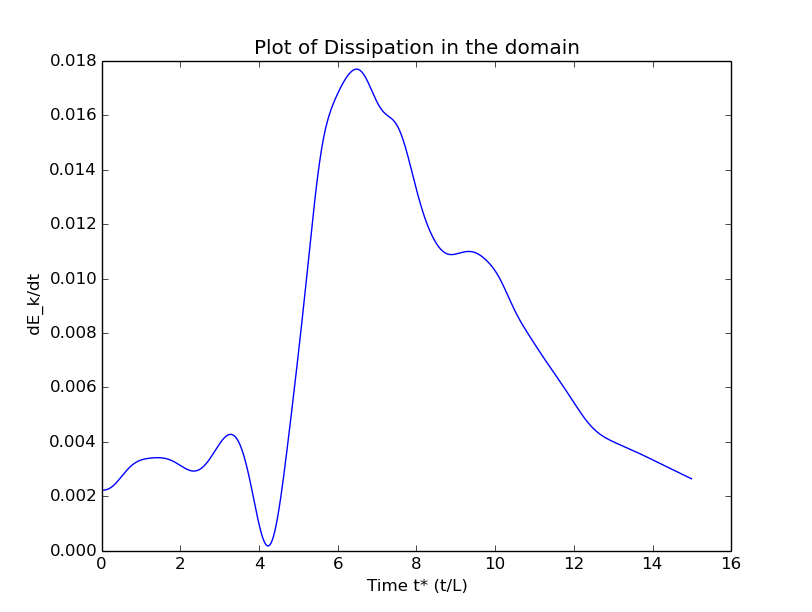
\includegraphics[scale=0.6]{3D/dissi.png}
\end{figure}


\end{document}
